\begin{figure}[!ht]
    \centering
    \begin{minipage}{.45\textwidth}
        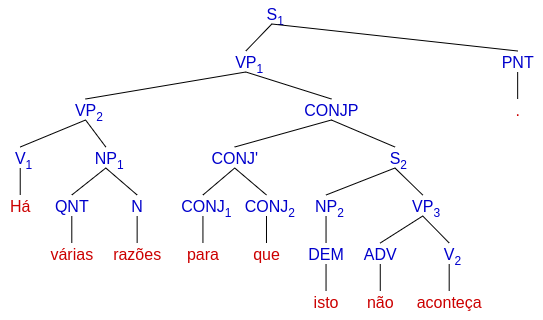
\includegraphics[width=\linewidth]{imagens/ec_cintil_conjp_tree_orig.png}
        \caption{árvore original}
    \end{minipage}
    \hfill
    \begin{minipage}{.45\textwidth}
        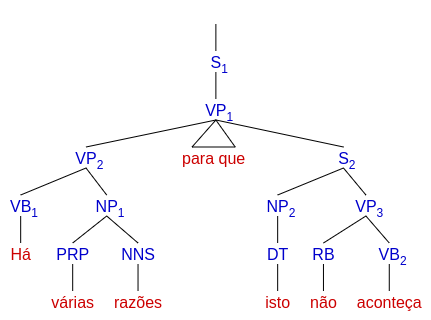
\includegraphics[width=\linewidth]{imagens/ec_cintil_conjp_tree_trans.png}
        \caption{árvore transduzida}
    \end{minipage}
    \hfill
    \vskip\floatsep
    \begin{minipage}{.45\textwidth}
        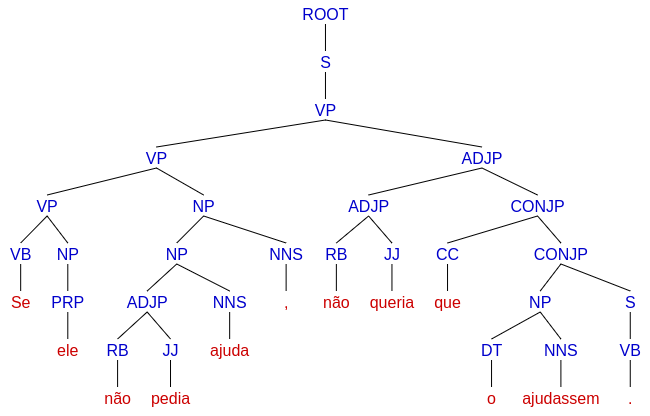
\includegraphics[width=\linewidth]{imagens/ec_cintil_conjp_tree_sp.png}
        \caption{árvore gerada pelo SP}
    \end{minipage}
    \caption[Estudo de caso CINTIL - Árvore da sentença transduzida com CONJP]{Estudo da sentença eCTMP-001150/117736, \textquote{Há várias razões para que isto não aconteça.}, que possui CONJP internamente.}
    \label{fig:ec_cintil_conjp_tree}
\end{figure}
    % \begin{minipage}[t]{.45\textwidth}
    % \scalebox{0.6}{
    %     \begin{forest}
    %     [
    %      [S 
    %       [S 
    %       [VP 
    %         [\textbf{CONJP} 
    %          [\textbf{CONJP} 
    %           [\textbf{CC Se}]
    %           [S 
    %           [NP 
    %             [PRP ele]
    %           ]
    %           [VP 
    %             [VP 
    %              [RB não]
    %              [\textbf{VB pedia}]
    %             ]
    %             [NP 
    %              [NNS ajuda]
    %             ]
    %           ]
    %           ]
    %          ]
    %         ]
    %         [VP 
    %          [VP 
    %           [RB não]
    %           [\textbf{VB queria}]
    %          ]
    %          [CONJP 
    %           [CC que]
    %           [\textbf{S} 
    %           [VP 
    %             [NP 
    %              [PRP o]
    %             ]
    %             [VB ajudassem]
    %           ]
    %           ]
    %          ]
    %         ]
    %       ]
    %       ]
    %      ]
    %     ]
    %     \end{forest}
    %     }
    % \end{minipage}
    % % 
    % \begin{minipage}[t]{.45\textwidth}
    %     \scalebox{0.6}{

    %     \begin{forest}
    %     [ROOT
    %       [S
    %         [VP
    %           [VP
    %             [VP [VB Se]
    %               [NP [PRP ele]]]
    %             [NP
    %               [NP
    %                 [ADJP [RB não] [JJ pedia]]
    %                 [NNS ajuda]]
    %               [\textbf{NNS ,}]]]
    %           [ADJP
    %             [ADJP [RB não] [\textbf{JJ queria}]]
    %             [CONJP [CC que]
    %               [\textbf{CONJP}
    %                 [NP [\textbf{DT o}] [\textbf{NNS ajudassem}]]
    %                 [S [\textbf{VB .}]]]]]]]]
    %     \end{forest}
    %     }
    % \end{minipage}